\documentclass{school-22.101-notes}
\date{October 24, 2011}

\begin{document}
\maketitle

\lecture{Nucleon-Nucleon Scattering}
We have discussed the bound state of a deuteron (a neutron plus a proton) in Chapter~\ref{2H-bound-state}. To gain more insights for the essential properties of nuclear force, we will look at scattering of a neutron by a proton, in particular taking into account the l-s coupling in $V_{\mathrm{nuc}}$. 


For this chapter, we are going to use relations, 
\begin{itemize}
\item QM flux: 
  \eqn{ \vec{J} = \frac{i \hbar}{2 \mu} (\psi \gradient \psi^* - \psi^* \gradient \psi) }
  For instance, in spherical coordinate system, 
  \eqn{ \vec{J} &= \frac{\hbar}{2 i m} \left[ \psi^* \gradient \psi - \psi \gradient \psi^* \right] = \frac{\hbar}{2 \mu i} \left[ \psi^* \dpsidr - \psi \dpsidr^* \right] }
\item Mass conservation: 
  \eqn{ \ddt (\psi^* \psi) + \divergence \vec{J} = 0 }
\end{itemize}


Reference: Krane 4.2, 11.8., Liboff 14.1.






\topic{Scattering Cross Sections}
Recall that the scattering cross-section of neutron from proton is around 20 barns for $1 \sim 10^6$ eV \footnote{it is not till we introduce spin-spin coupling that we can explain this high scattering cross section}. 

To derive relations about the scattering cross section, we start by defining the incoming wave as a planar wave, and the outgoing wave as a spherical one. We define the scattering amplitude $f(\theta)$ as in $\psi_{\mathrm{sc}} = f(\theta) \frac{e^{i (\uline{k} \uline{r} - wt)}}{r}$. 
\begin{align}
\psi_{\mathrm{inc}} &= e^{i (\uline{k} \uline{r} - wt)} = e^{ikz}  = e^{ikr \cos \theta} 
&J_{\mathrm{inc}} &= \frac{\hbar k}{\mu} \\
\psi_{\mathrm{sc}} &=  f(\theta) \frac{e^{i (\uline{k} \uline{r} - wt)}}{r} = f(\theta) \frac{e^{ikr}}{r} &J_{\mathrm{sc}} &= \frac{\hbar k}{\mu r^2} |f(\theta)|^2 \\
\sigma(\theta) &= \mbox{Angular Differential xs} = \dsigmadOmega  &\sigma &= \int \sigma(\theta) \dOmega
\end{align}






Cross section is the probability that an incoming wave scatters along the solid angle $\Omega+\dOmega$. If we specify a small area on the spherical surface along the solid angle $\Omega$, then we can represent the area with $\Omega$:
\begin{align}
\dA &= r^2 \dOmega = r^2 \sin \theta \dtheta \dphi \\
\dsigma J_{\mathrm{inc}} &= J_{\mathrm{sc}} \dA = J_{\mathrm{sc}} r^2 \dOmega \\
\dsigmadOmega &= \frac{J_{\mathrm{sc}} r^2}{J_{\mathrm{inc}}} = \sigma(\theta) 
\end{align}

In the limit of $r \to \infty$, 
\eqn{ \psi &\approx e^{ikr \cos \theta} + f(\theta) \frac{e^{ikr}}{r} }
\eqn{ J_r &\approx \frac{|f(\theta)|^2}{r^2} \frac{\hbar k}{\mu}  & \Rightarrow r^2 \dOmega J_r &= |f(\theta)|^2 J_{in}}
We can derive the relation for differential scattering cross section $\dsigmadOmega$ and the total scattering cross section $\sigma$, 
\begin{align}
\left. \begin{array}{c}
J_{\mathrm{inc}} = \frac{\hbar k}{\mu} b^2  \\
J_{\mathrm{sc}} = \frac{\hbar k}{\mu r^2} b^2 |f(\theta)|^2 \\
\end{array} \right\} & \Rightarrow \boxed{\dsigmadOmega =  \frac{J_{\mathrm{sc}} r^2}{ J_{\mathrm{inc}}} = |f(\theta)|^2 }  \\
\Aboxed{ \sigma &= \int \dOmega |f(\theta)|^2  = 2 \pi \int_{\pi}^0 \derivative \cos \theta |f(\theta)|^2 }
\end{align}
Notes of scattering amplitude $f(\theta)$: 
\begin{enumerate}
\item $f(\theta)$ is scattering intensity as a function of scattering angle.
\item Generally $f(\theta)$ is anisotropic. For $l=0$ though there is no angular dependency, $f(\theta) \to $ constant. 
\item Angular differential xs $\sigma(\theta)$ is proportional to the scattering amplitude squared. Total scattering cross section is just angular differential cross section integrated over all angles.  
\item To solve for $f(\theta)$, use Method of Partial Waves. The result is in Eq.~\ref{f-theta}. 
\end{enumerate}




\topic{Method of Partial Waves, Phase Shifts} 
To find $f(\theta)$, we solve the Schrodinger Equation for wave function $\psi(\uline{r}, t) = \psi(\uline{r}) e^{-iEt/\hbar}$:
\eqn{\left[ - \frac{\hbar^2}{2 \mu} \uline{\gradient}^2 + V(\uline{r}) \right] \psi (\uline{r}) = E \psi(\uline{r}) }
We've already solved for this problem for the bound state condition ($E <0$), whereas now we consider the scattering case $E>0$, with the boundary condition:
\eqn{\psi(r) \xrightarrow{r \gg r_0} \psi_{\mathrm{inc}} + \psi_{\mathrm{sc}} = e^{i \uline{k r}} + f(\theta) \frac{e^{ikr}}{r} \label{BC}}

\begin{enumerate}
\item Set-up Partial Wave: we expand the $\psi(r)$ into $\psi(r, \theta)$, notice there is no $\phi$ dependence because of $V(r)$. Then we can write $\psi(r,\theta)$ into the summation of partial waves, in which $P_l (\cos \theta)$ is the Legende Polynomial, 
\eqn{\psi(r,\theta) = \Sum_{l=0}^{\infty} R_l(r) P_l (\cos \theta) }

\item Simplify Schrodinger Equation, consider radial function: 
\begin{align}
\left. \begin{array}{c}
\left(- \frac{\hbar^2}{2 \mu} \uline{\gradient}^2 + V(\uline{r}) - E  \right) \psi(r,\theta) = 0 \\
u_l (r) = r R_l (r) 
\end{array} \right\} 
\left( -\frac{\hbar^2}{2 \mu} \pprn2 +\frac{\hbar^2 l(l+1)}{2 \mu r^2} + V(\uline{r}) - E  \right) u_l (r) &= 0 \\
\left( \pprn2 - \frac{l(l+1)}{r^2} - \frac{2\mu}{\hbar^2} V(\uline{r}) + \overbrace{\frac{2\mu}{\hbar^2} E}^{\to k^2}  \right) u_l (r) &= 0 
\end{align}

\item For $r\le r_0$, $V(r) \neq 0$: we don't actually pursue this case. Indeed, we only consider the extreme case $V (r) =0$. 
\begin{align}
\left( \pprn2 - \frac{l(l+1)}{r^2} - \frac{2\mu}{\hbar^2} V(\uline{r}) + k^2  \right) u_l (r) &= 0 
\end{align}

\item For $r>r_0$, $V(r) =0$: $j_l (kr)$ are Spherical Bessel Functions, and $n_l (kr)$ are Spherical Neumann Functions:
\begin{align}
\left( \pprn2 - \frac{l(l+1)}{r^2} + k^2  \right) u_l (r) &= 0  & u_l (r) &= B_l r j_l (kr) + C_l r n_l (kr)  \\
j_l (x) &\xrightarrow{x \gg 1} \frac{1}{x} \sin \left( x - \frac{l \pi}{2} \right) & n_l (x) &\xrightarrow{x \gg 1} - \frac{1}{x} \cos \left( x - \frac{l \pi}{2} \right) 
\end{align}
For the extreme case $r \gg r_0, kr \gg 1$, then we can apply our Boundary Condition: 
\eqn{ u_l (r) \xrightarrow{kr \gg 1} \frac{B_l}{k} \sin \left( kr - \frac{l \pi}{2} \right) - \frac{C_l}{k} \cos \left( kr - \frac{l \pi}{2} \right)  = \frac{A_l}{k} \sin \left( kr - \frac{l \pi}{2} + \delta_l \right) \label{delta_l}}
in which $ \delta_l = \mbox{phase shift of each partial wave after interact with $V(r)$} $
\eqn{ \boxed{ \psi(r,\theta) \xrightarrow{kr \gg 1} \Sum_{l=0}^{\infty} \frac{A_l}{kr} \sin \left( kr - \frac{l \pi}{2} + \delta_l \right) P_l (\cos \theta) \label{sol} } }
Eq.~\ref{sol} is the solution to the Schrodinger Equation for the extreme of $kr \gg 1$. 

Keep in mind that we are after $f(\theta)$, and we will apply the BC we defined above to solve for $f(\theta)$. 
\end{enumerate}


\topic{Phase Shifts}
A phase shift $\delta_l$ is defined in the above section in Eq.~\ref{delta_l}. We can determine $\delta_l$ analytically \footnote{try using the trigonometry $\sin(a+b) = \sin(a) \cos (b) + \cos(a) \sin(b)$?}. Keep in mind that $\delta_l$ is the phase shift for each of the partial wave that can scatter. It is a result of a partial wave interacting with the potential.  
\begin{figure}[ht]
    \centering
    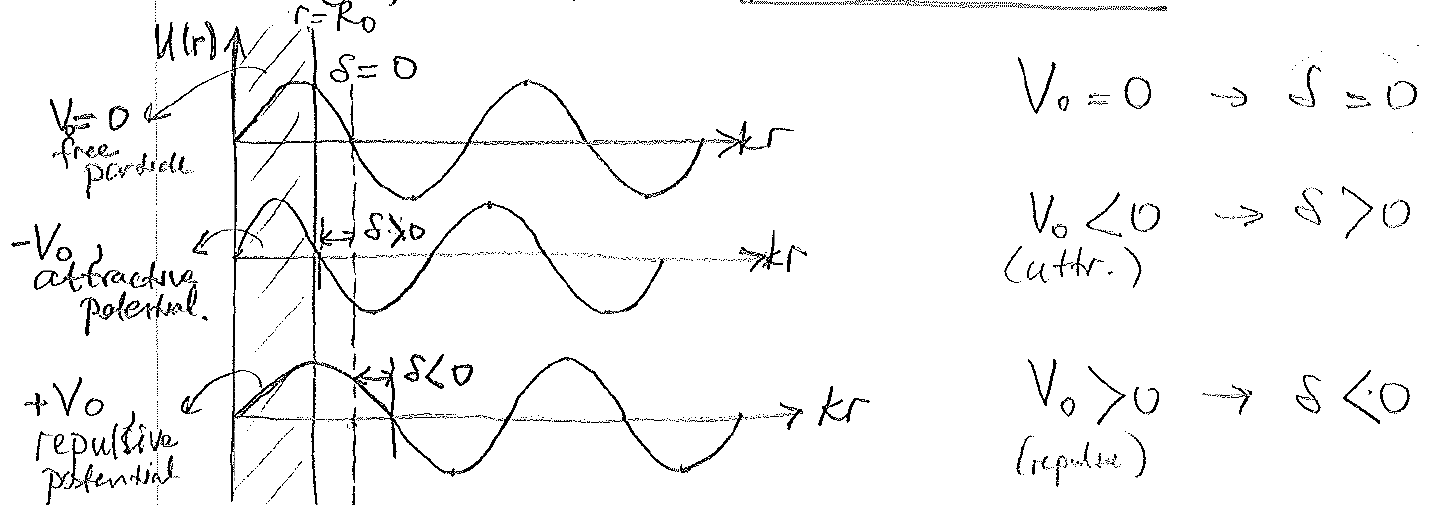
\includegraphics[width=4.5in]{images/scattering/scattering-potential-phase-shift.png}
    \caption{Phase Shift, Scattering Length }
\end{figure}

\topic{Angular Differential Cross Section $\sigma (\theta)$, Total Cross Section $\sigma$}
Start with the solution of Schroedinger equation after partial wave expansion as in Eq.~\ref{sol}, we apply BC Eq.~\ref{BC}. To do so, we need to expand two terms: 
\begin{itemize}
\item $ f(\theta) = \Sum_{l=0}^{\infty} f_l P_l (\cos \theta)$.
\item $e^{ikz} = e^{ikr \cos \theta} \xrightarrow{kr \gg 1} \Sum_l  \frac{i^l (2l+1)}{kr} \sin \left( kr - \frac{l \pi}{2} \right) P_l (\cos \theta) = \Sum_l  \frac{i^l (2l+1)}{kr} \frac{1}{2i} \left[ e^{ i \left( kr - \frac{l \pi}{2} \right)} - e^{ -i \left( kr - \frac{l \pi}{2} \right)} \right] P_l (\cos \theta)$. 
\end{itemize}
Then we equate the coefficient before the same $l$ state, and solve for $f(\theta)$ as: 
\begin{align}
f(\theta) &= \frac{1}{k} \Sum_{l=0}^{\infty} (2l+1) e^{i \delta_l} \sin \delta_l P_l (\cos \theta) \label{f-theta} \\
\sigma (\theta) &= |f(\theta)|^2 = \frac{1}{k^2} \left| \Sum_{l=0}^{\infty} (2l+1) e^{i \delta_l} \sin \delta_l P_l (\cos \theta) \right|^2 \label{sigma-theta} \\
\sigma &= \int  \sigma(\theta) \dOmega= \frac{4 \pi}{k^2} \Sum_{l=0}^{\infty} (2l+1) e^{i \delta_l} \sin^2 \delta_l  \label{sigma} 
\end{align}
Notice, Eq.~\ref{f-theta} $\sim$ Eq.~\ref{sigma} are the general expression. In the example demonstrated below, we are going to consider some cases that the above solutions simplify. 

\end{document}
